\documentclass{homework}

\title{Homework 10}

\newcommand{\arcsinh}{\mathrm{arcsinh}}

\begin{document}
    \maketitle

    \problem
    % TODO Prove existence

    \problem
    Denote
    \[A_t:=-\int_0^tg(s)\diff W_s+\frac{1}{2}\int_0^tg^2(s)\diff s\]
    then $A_t$ is an It\^o process as
    \[\diff A_t=-g(t)\diff W_t+\frac{1}{2}g^2(t)\diff t\]
    hence
    \[\begin{aligned}
        \diff I_t&=\diff \e^{A_t}\\
        &=\e^{A_t}\left(\diff A_t+\frac{1}{2}(\diff A_t)^2\right)\\
        &=\e^{A_t}(-g(t)\diff W_t+g^2(t)\diff t)\\
        &=I_t(-g(t)\diff W_t+g^2(t)\diff t)
    \end{aligned}\]
    It follows that
    \[\diff I_t\diff X_t=-\e^{A_t}g^2(t)X_t\diff t=-I_tX_tg^2(t)\diff t\]
    therefore,
    \[\begin{aligned}
        &\diff(I_tX_t)\\
        =&I_t\diff X_t+X_t\diff I_t+\diff I_t\diff X_t\\
        =&I_tf(t,X_t)\diff t+I_tg(t)\diff W_t+I_tX_t(-g(t)\diff W_t+g^2(t)\diff t)
        -I_tX_tg^2(t)\diff t\\
        =&I_tf(t,X_t)\diff t
    \end{aligned}\]

    \problem
    \begin{subproblem}[(\alph*)]
        \item
        We have that
        \[f(t,X_t)=0,g(t)=\alpha\]
        thus
        \[I_t=\e^{-\alpha W_t+\alpha^2t/2}\]
        and
        \[\diff(I_tX_t)=0\]
        which gives us
        \[I_tX_t=I_0X_0=X_0\]
        i.e.,
        \[X_t=\frac{X_0}{I_t}=X_0\e^{\alpha W_t-\alpha^2t/2}\]

        \item
        $I_t$ and following ones are the same as above
        since $g(t)=\alpha$ is not changed.
        And we have that $f(t,X_t)=r$, hence
        \[\diff(I_tX_t)=rI_t\diff t\]
        Therefore,
        \[\begin{aligned}
            X_t&=I_t^{-1}\left(I_0X_0+r\int_0^tI_s\diff s\right)\\
            &=X_0\e^{\alpha W_t-\alpha^2/t}+r\int_0^t\e^{\alpha(W_t-W_s)-\alpha^2(t-s)/2}\diff s
        \end{aligned}\]

        \item
        We have that $f(t,X_t)=X_t$, thus
        \[\diff(I_tX_t)=I_tX_t\diff t\]
        Therefore,
        \[I_tX_t=I_0X_0\e^t=X_0\e^t\]
        as the quadratic variation
        \[\diff(I_t^2X_t^2)=0\]
        i.e.,
        \[X_t=X_0\e^{\alpha W_t-(\alpha^2/2-1)t}\]

        \item
        We have that $f(t,X_t)=1/X_t$, thus
        \[\diff Y_t=\diff(I_tX_t)=\frac{I_t\diff t}{X_t}
        =\frac{I_t^2\diff t}{Y_t}\]
        i.e.,
        \[Y_t\diff Y_t=I_t^2\diff t\]
        Therefore,
        \[\int_0^tY_s\diff Y_s=\frac{Y_t^2-Y_0^2}{2}=\int_0^tI_s^2\diff s\]
        i.e.,
        % TODO X0 > 0 cancels minus sign ?
        \[\begin{aligned}
            X_t&=\pm I_t^{-1}\sqrt{Y_0^2+2\int_0^tI_s^2\diff s}\\
            &=\pm\sqrt{X_0^2\e^{2\alpha W_t-\alpha^2t}
            +2\int_0^t\e^{-2\alpha(W_s-W_t)+\alpha^2(s-t)}\diff s}
        \end{aligned}\]

    \end{subproblem}

    \problem
    Here we plot the graph of a path of $X_t=1/(1-W_t)$, see \cref{fig:blowup}.
    \begin{figure}[h]
        \centering
        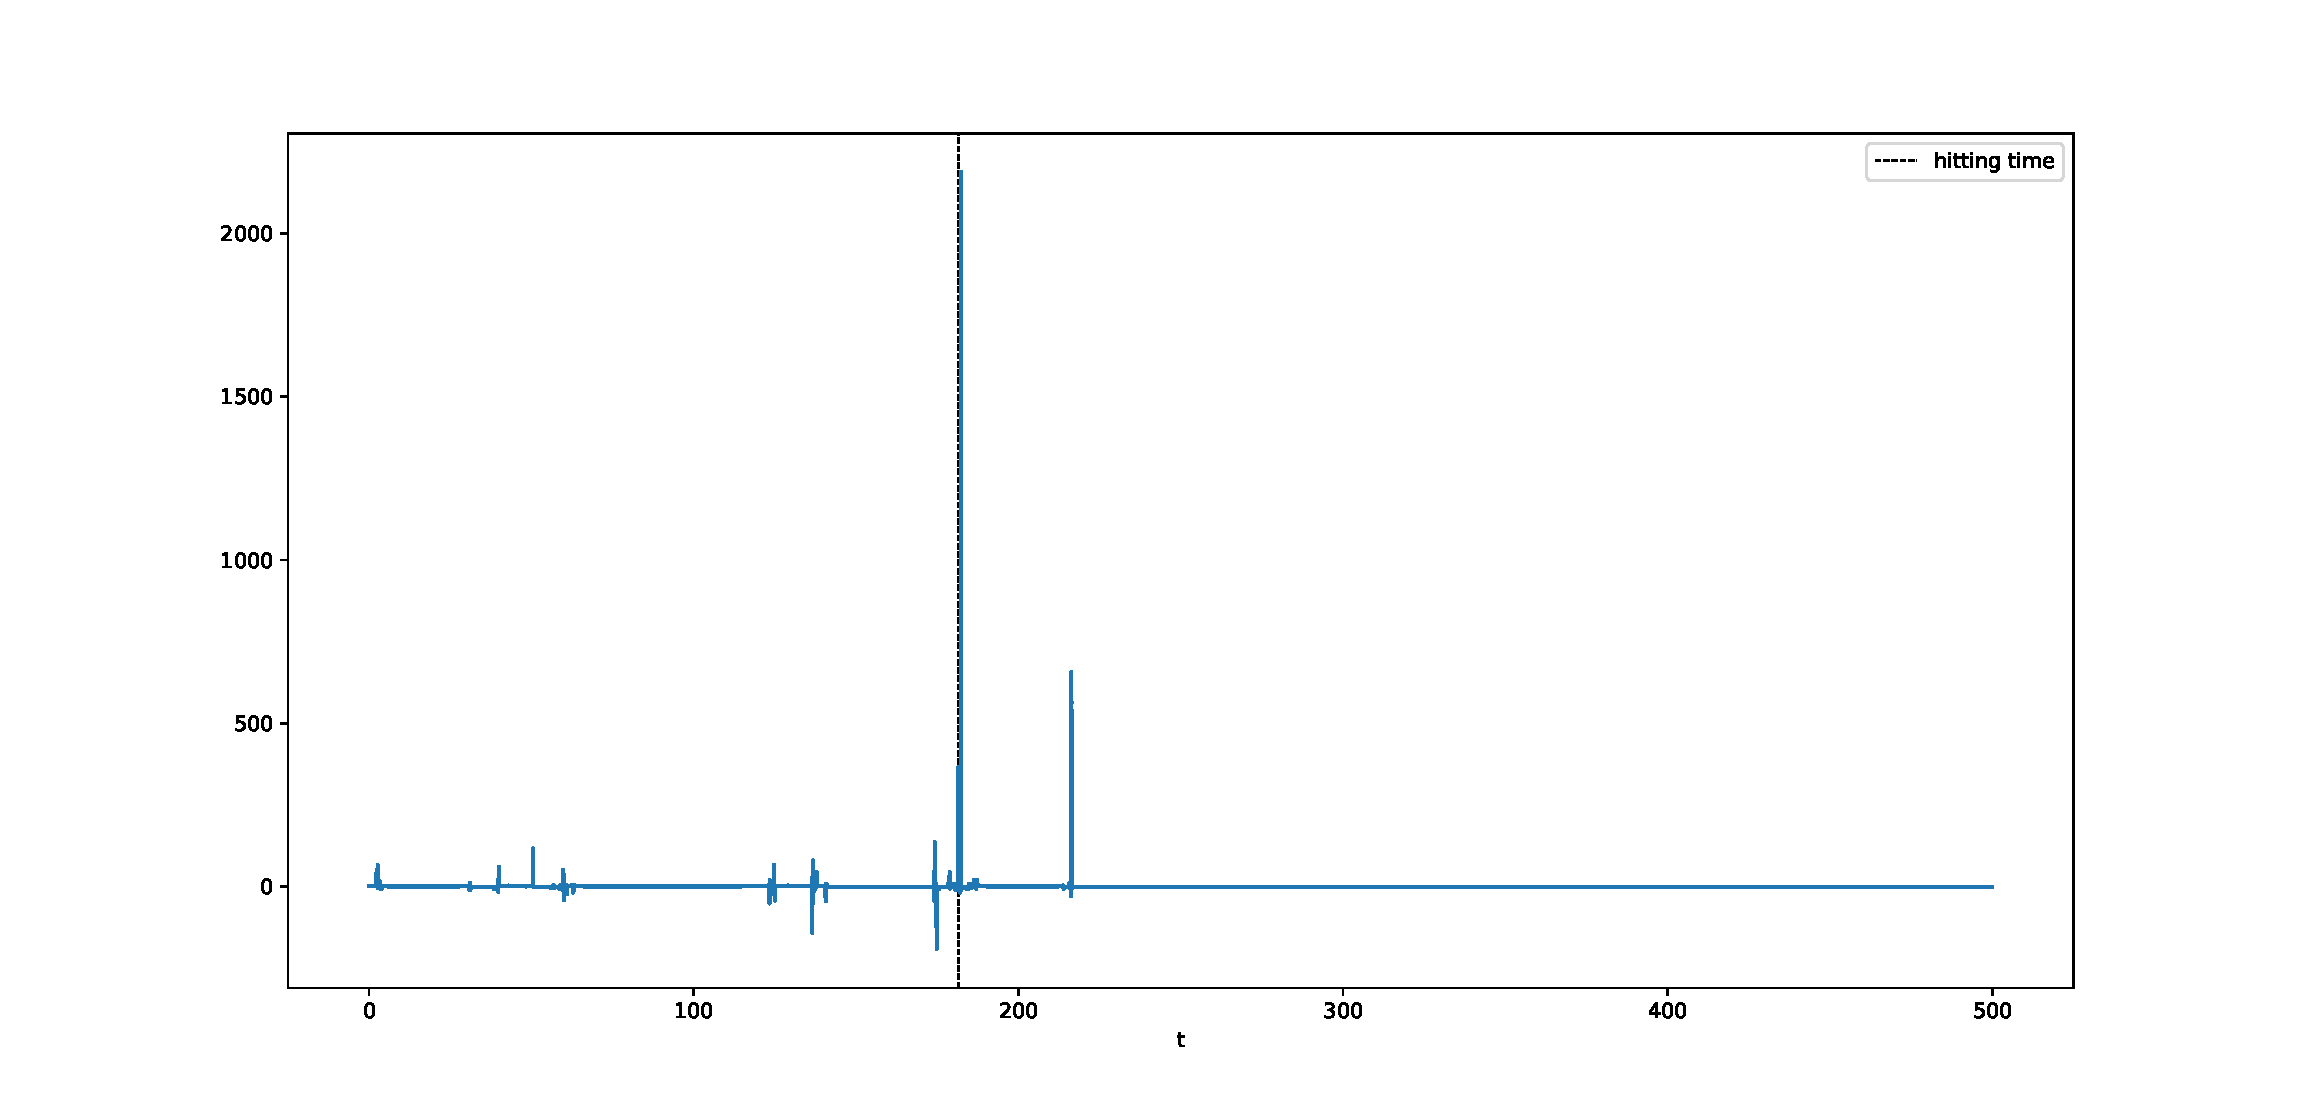
\includegraphics[width=\textwidth]{blowup}
        \caption{Blow-up}
        \label{fig:blowup}
    \end{figure}

    \problem
    \begin{subproblem}[\roman*)]
        \item
        We have from Taylor's expansion that
        \[\diff X_t=\diff\left(\frac{1}{1-W_t}\right)
        =\frac{\diff W_t}{(1-W_t)^2}
        +\frac{1}{2}\frac{2(\diff W_t)^2}{(1-W_t)^3}
        =X_t^2\diff W_t+X_t^3\diff t\]
        and apparently $X_0=1/(1-W_0)=1$.

        \item
        Denote $X_t=f(t,W_t)$, then we have from It\^o's lemma that
        \[\diff X_t=\left(f_t+\frac{f_{xx}}{2}\right)\diff t+f_x\diff W_t\]
        where $f_t$ is short for $\partial f(t,W_t)/\partial t$, $f_{xx}$ for
        $\partial^2 f(t,W_t)/\partial W_t^2$, etc.

        It follows that
        \[f_x=f^2,f_t+\frac{f_{xx}}{2}=f^3\]
        The first equation gives us
        \[f_{xx}=2ff_x=2f^3\]
        Substituting this into the second one gives us
        \[f_t+f^3=f^3\]
        i.e., $f_t=0$.
        Therefore $f_x=f^2$ is an ODE actually, to which the solution is
        \[f(t,W_t)=\frac{1}{C-W_t}\]
        And initial condition $X_0=1$ yields $C=1$, hence
        \begin{equation}
            \label{eq:blow sol}
            X_t=\frac{1}{1-W_t}
        \end{equation}
        With the uniqueness of the SDE, we can conclude that
        the solution is \cref{eq:blow sol}.

        \item
        See \cref{fig:blowup}.

        \item
        We use the average of trials to estimate the expectation.
        After trials of 1000 times with maxtime\marginnote{
            Given an finite time, chances are that the path
            does not hit the line, so we choose the
            hitting time to be assigned to the maxtime.
            And we adjust the maxtime to see the difference
            (the ideal occasion is that the
            maxtime is infinite).

            Actually, we know that the expectation of hitting time of Brownian
            motion is infinite, i.e.,
            \[E(\inf{\{t:W_t=m\}})=\infty,m\in\mathbb R\]
        } 1000, 5000, 10000,
        we have an estimate
        of 385.5, 1029.2, 1425.4 accordingly. See \cref{fig:dist}
        for the distributions.
        \begin{figure}[h]
            \centering
            \begin{subfigure}[b]{0.3\textwidth}
                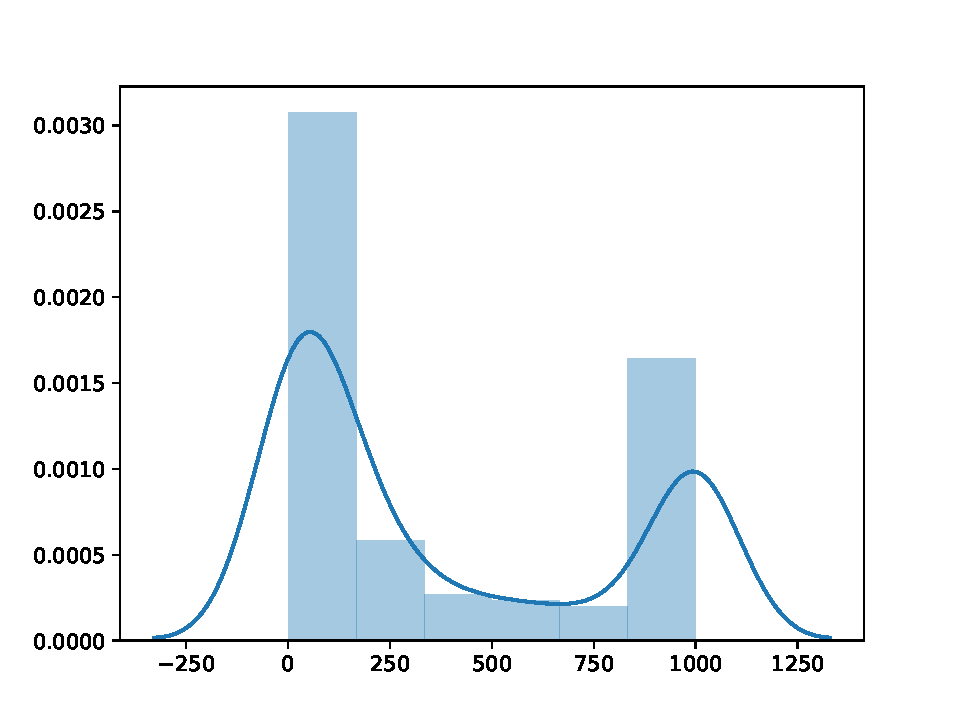
\includegraphics[width=\textwidth]{max=1000}
                \caption{Maxtime 1000}
            \end{subfigure}
            \begin{subfigure}[b]{0.3\textwidth}
                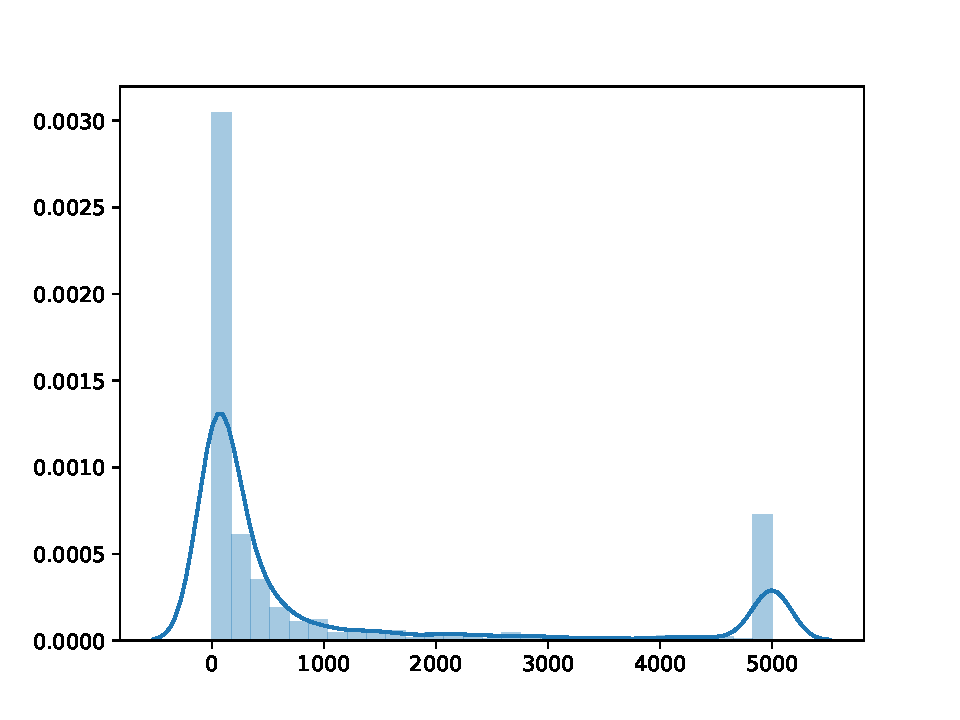
\includegraphics[width=\textwidth]{max=5000}
                \caption{Maxtime 5000}
            \end{subfigure}
            \begin{subfigure}[b]{0.3\textwidth}
                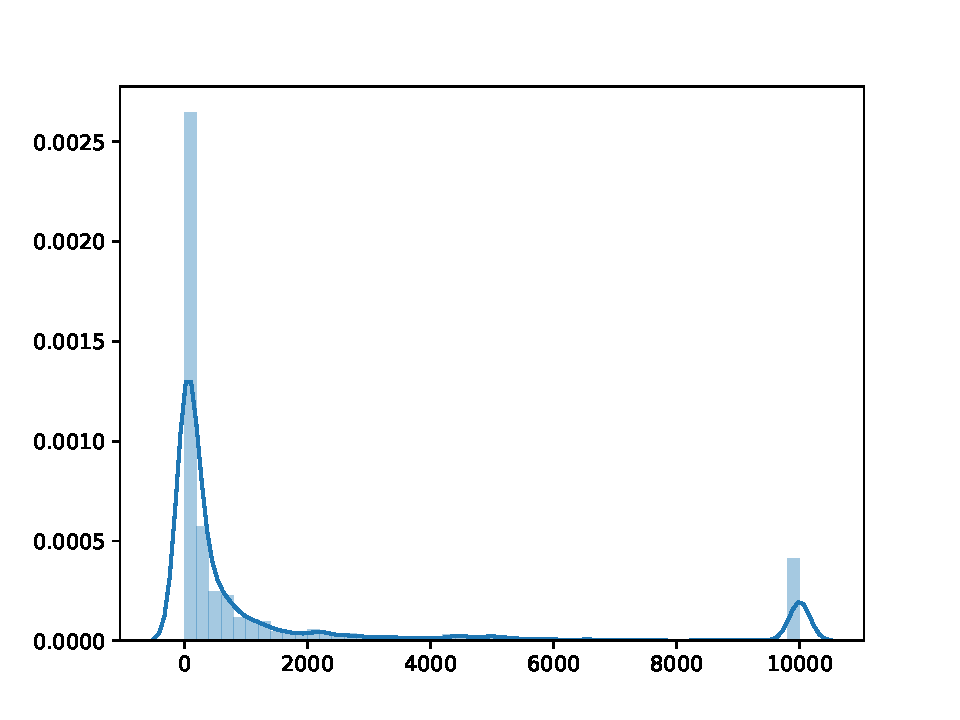
\includegraphics[width=\textwidth]{max=10000}
                \caption{Maxtime 10000}
            \end{subfigure}
            \caption[][2.53cm]{Distribution of hitting time with different max time}
            \label{fig:dist}
        \end{figure}
    \end{subproblem}

    \problem
    \begin{subproblem}
        \item
        % TODO Prove uniqueness

        \item
        Denote\sidenote{The solution is from
        \url{https://math.stackexchange.com/questions/915394/solve-dx-t-sqrt1x-t2-frac12x-t-dt-sqrt1x-t2-dw-t}}
        $\sigma(x):=\sqrt{1+x^2}$, then
        \[\diff X_t=(\sigma(X_t)+X_t/2)\diff t+\sigma(X_t)\diff W_t\]
        And denote $Z_t:=f(X_t)$, where
        \[f(x)=\int_0^x\frac{1}{\sigma(y)}\diff y\]
        then we know that
        \[f'(x)=\frac{1}{\sigma(x)},f''(x)=-\frac{\sigma'(x)}{\sigma^2(x)}\]
        And we have from It\^o's lemma that
        \[\begin{aligned}
            \diff Z_t&=\diff f(X_t)\\
            &=f'(X_t)\diff X_t+\frac{1}{2}f''(X_t)(\diff X_t)^2\\
            &=\left(\frac{f''\sigma^2}{2}
            +\left(\sigma+\frac{X_t}{2}\right)f'\right)\diff t
            +f'\sigma\diff W_t\\
            &=\left(-\frac{\sigma'}{2}+\frac{X_t}{2\sigma}+1\right)\diff t+\diff W_t
        \end{aligned}\]
        where $f$ is short for $f(X_t)$, $\sigma$ for $\sigma(X_t)$ etc.
        But do note that $X_t/\sigma=X_t/\sqrt{1+X_t^2}=\sigma'$, then
        we obtain that
        \[\diff Z_t=\diff t+\diff W_t\]
        which gives us
        \[Z_t=Z_0+t+W_t=f(x_0)+t+W_t\]
        Indeed, one can show that $f(x)=\arcsinh x$
        thus we obtain $X_t$ as
        \[\begin{aligned}
            X_t&=\sinh Z_t\\
            &=\sinh(\arcsinh x_0+t+W_t)\\
            &=x_0\cosh(t+W_t)+\sqrt{1+x_0^2}\sinh(t+W_t)
        \end{aligned}\]
    \end{subproblem}

\end{document}